\section{Conclusions}

In this work we introduced a model for a system to learn proper handover settings for objects through observations of handovers performed by humans. We showed that we can classify objects depending on a set of features extracted at the moment of the handover. By training a network to output a handover class based on an image of an object we also showed that the objects that have been assigned the same class share similar visual features. Last we showed that these features that have been learned also scale well to other sets of objects that are new to the system.

Based on the features extracted from the handovers, the system is able to cluster the objects and classify them. A handover class will then be defined by a set of features that are to be applied to an object when handing it over. Before clustering we performed PCA to identify the dominant features which were: ratio of object covered by the grasp, direction of vector between center of mass of the object and center grasp in y-axis and in x-axis. Two main classes were identified, where one class contained larger cylindrical objects used for containing for example liquids (cup, glass, bottle, etc.) that were handover in a similar fashion, while objects that are thinner and have a distinct usage area (hammer, pen, scissors) had a different set of features. Outliers in the training set were clustered into their own classes (cutters, box and tube) that contained unique attributes for these objects.

Color and depth images were then taken of the objects from different angles. The blue channel was replaced with the depth image, and then used for training a CNN to recognize the objects and output their respective handover class. The classes that contained only one object were discarded as they would not contain enough data to properly train to identify them. The resulting network was then tested on a different set of images of objects that resembled the training set and manually labeled after the two main classes were created.

Mean performance for our network is 90.6\% with a standard deviation of 1.3\% for objects that were new to the system, while 99.8\% accuracy with a standard deviation of 0.3\% on objects it was trained on. We observed that the network became more biased for the first class than the second, which is likely due to the fact that the two classes were not completely balanced between the objects, suggesting that one class had more versatile features to learn from than the other. We note that the network had a hard time learning to recognize objects made of glass, probably because of troubles with the infrared sensor in the depth camera refracting on the material while taking pictures, making them more challenging to recognize. Objects in the same class but made of other material had results close to 100\%, as well as the objects from the first class which confirms our hypothesis that objects with similar geometry are handed over in similar fashion. In overall the results are quite good considering the small dataset to train on and the artifacts that are created with the depth camera, and with a larger amount of objects and images better results could have probably been achieved. More ideas on how to improve this model are presented in section \ref{sec:future-work}.

\section{Future Work}
\label{sec:future-work}

The results of this work show that a system is able to autonomously learn to handover objects and adapt to novel ones, but some caveats do exist for it to become truly autonomous. The largest problem is object detection, which is a challenging field within computer vision. This work took help of AprilTags to locate and track the objects but in a live environment these tags do not exist on all objects and the system would need a better way of recognizing the object in the handover scene to extract data about the handover. Also in some cases the AprilTag itself could lead to awkward grips of the objects that can lead to incorrect data (see figure \ref{fig:fw_handover_awkward}). Some work show good success using alternatives such as point cloud libraries (\parencite{Chan2015a}). Object detection using point clouds was tried in this work before using AprilTags, but with very poor results. This is something that would need more work to try and implement better without the help of the tags.

\begin{figure}
	\centering
	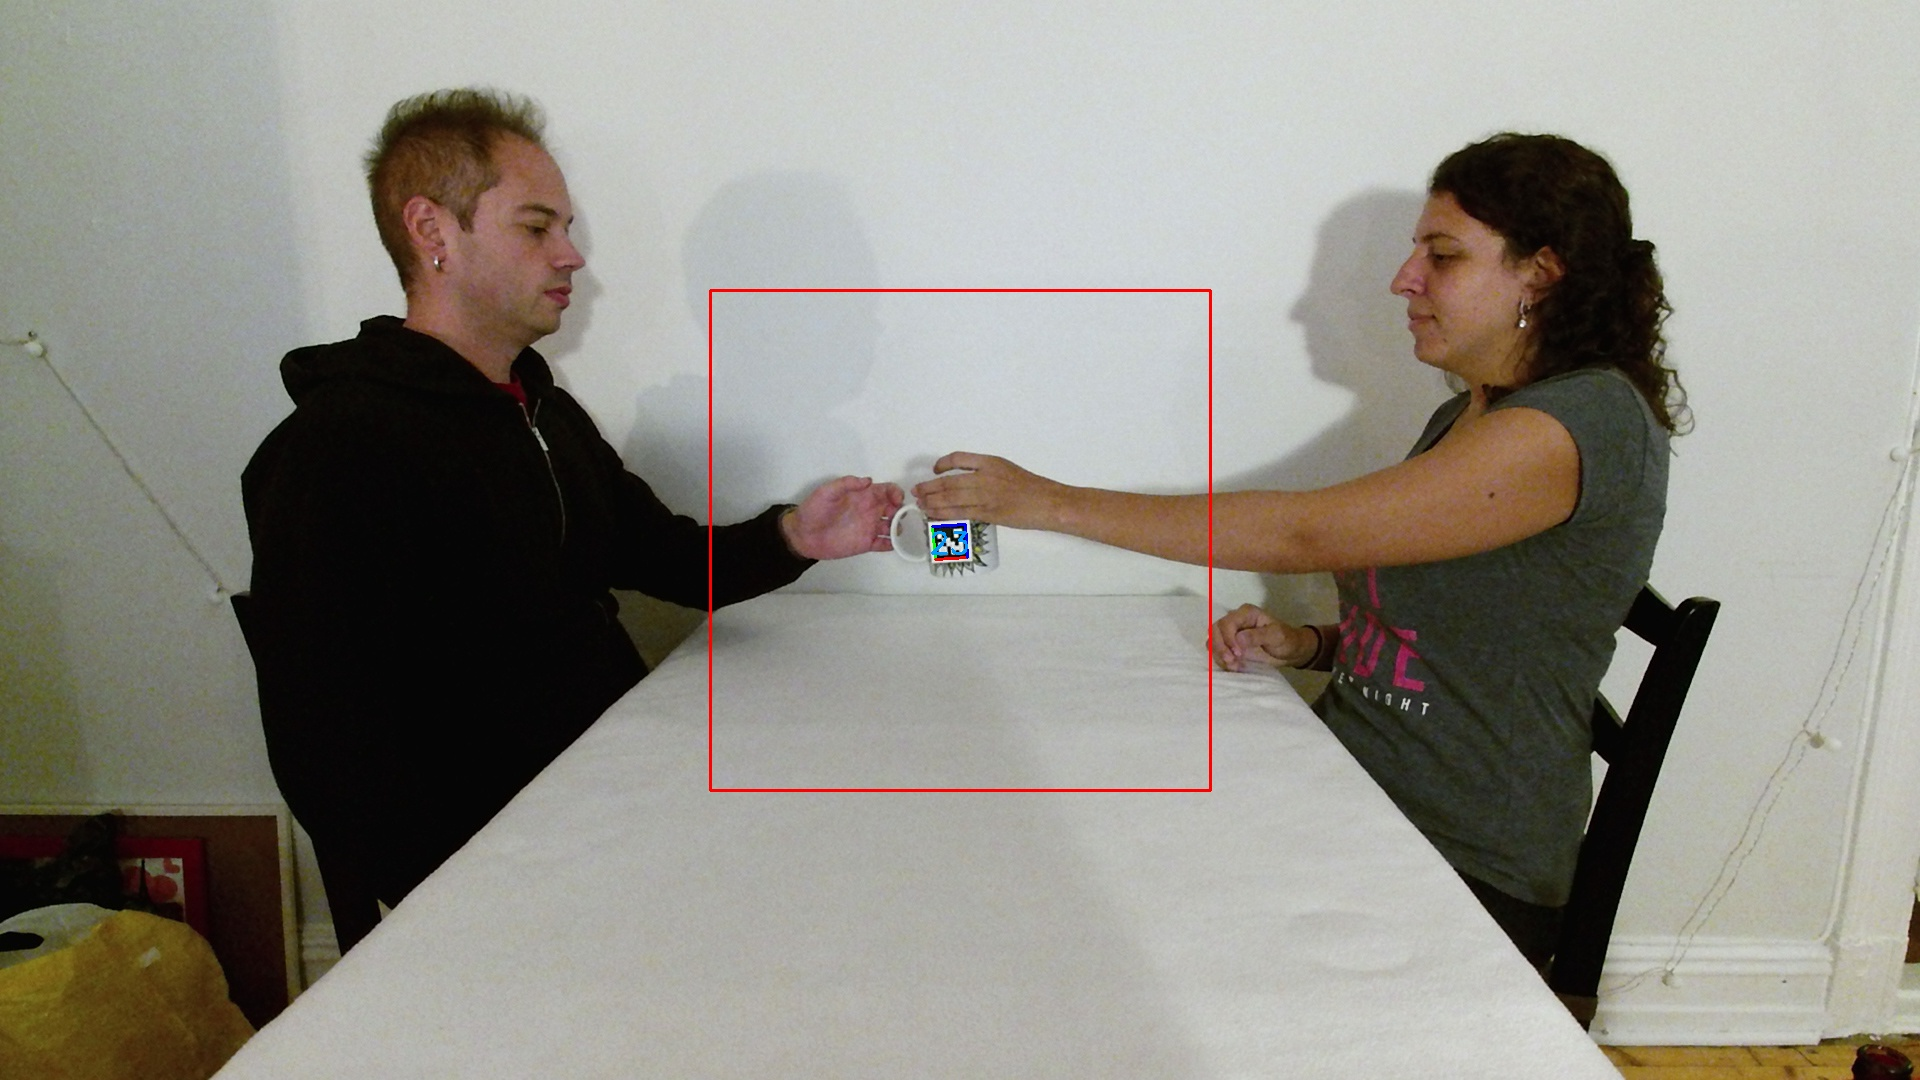
\includegraphics[width=\textwidth]{img/conclusion/awkward_handover_frame.jpg}
	\caption{Some grasps could become unnatural because of the AprilTags.}
	\label{fig:fw_handover_awkward}
\end{figure}

Handover classes from clustering are however not enough to tell a robot how to grasp an object when handing it over. As seen in the results when the settings of one class are applied to an object the grasp region can become outside of it, though rotation and direction from center of object are correct. Future work would have to include calculating more precisely where a robot can grasp the object when handing it over given the data from the handover class.
